\section{ SR0008ES23 }


\subsection{Meta}

    \textbf{Title:}
    Data science, analytics and artificial intelligence in e-health: trends, applications and challenges

    \begin{table}[H]
        \centering
        \begin{tabular}{|c|c|c|c|c|c|c|c|c|}
            \hline
                \textbf{Rank} & \textbf{Grasp} & \textbf{Grade} & \textbf{Type} & \textbf{Outcome} & \textbf{Domain} & \textbf{COV19} & \textbf{CoI} & \textbf{DB} \\
            \hline
                5 & 93\% & C & A & ?? & A & Yes & Yes & No \\
            \hline
        \end{tabular}
        \caption{Reference's metadata}
        \label{tab:SR0008ES23}
    \end{table}

\subsection{Summary}
    The review work by Juliana Castaneda et al. \cite{x249} is a general overview of AI practices in healthcare and their implementation. It considers the development of AI solutions due to the COVID-19 crisis. The paper qualitatively summarises the machine learning methods in the scope of data development and some relation to the Internet of Things technology. The practical side of the work is in the methods used for quantifying the frequency of the word's appearance in the studies and the automatic topic extraction script. This work will benefit most newcomers in the crossfield of Artificial intelligence and healthcare who want to decide on the direction of their research.

\subsection{Notes}
    \begin{itemize}
        \item Non-negative matrix factorization (NMF). Diverse data into meaningful topics.
        \item Data preprocessing + NMF + Python (scikit-learn library)
        \item Pyrthon cleaning data code \url{https://github.com/Julianac-j/NMF_ehealth}
    \end{itemize}


\subsection{Reading}
    \textbf{Abstract:}
    The development and application of the predictive models, and artificial intelligence in healthcare environment are hihglighted in this literature review. In addition the benefits for healthcare organisations will be discussed alongside the obsticles and complexities.
    
    \textbf{Page 2:}
    Introduction to Big Data technology, Machine Learning, and Artificial intelligance comparing with the progress similar to arise of the Internet.
    
    \textbf{Page 3:}
    The Big Data in scope of IoT Technology as well as IoT in Healthcare System were outlined in this page. The basic explanation of search methods for the literature and the structure of the article are presented next.
    
    \textbf{Page 4:}
    Here is shown an exponantial increas in papers regarding the AI, e-health, and data science in Scopus and Google Scholar with Google Scholar in the lied.
    
    \textbf{Page 5:}
    The authors mentioned the pandemic challenge and the responce in the scientific community to it. Also the non-negative matrix factorization was described with examples of implementation in the literature. In basic terms, this is method of extracting data from unstructured dataset into meaningful topics.
    
    \textbf{Page 6:}
    Using Python clean the data, define the workd frequency and using NMF quantify the most common topics.
    \begin{figure}[H]
        \centering
        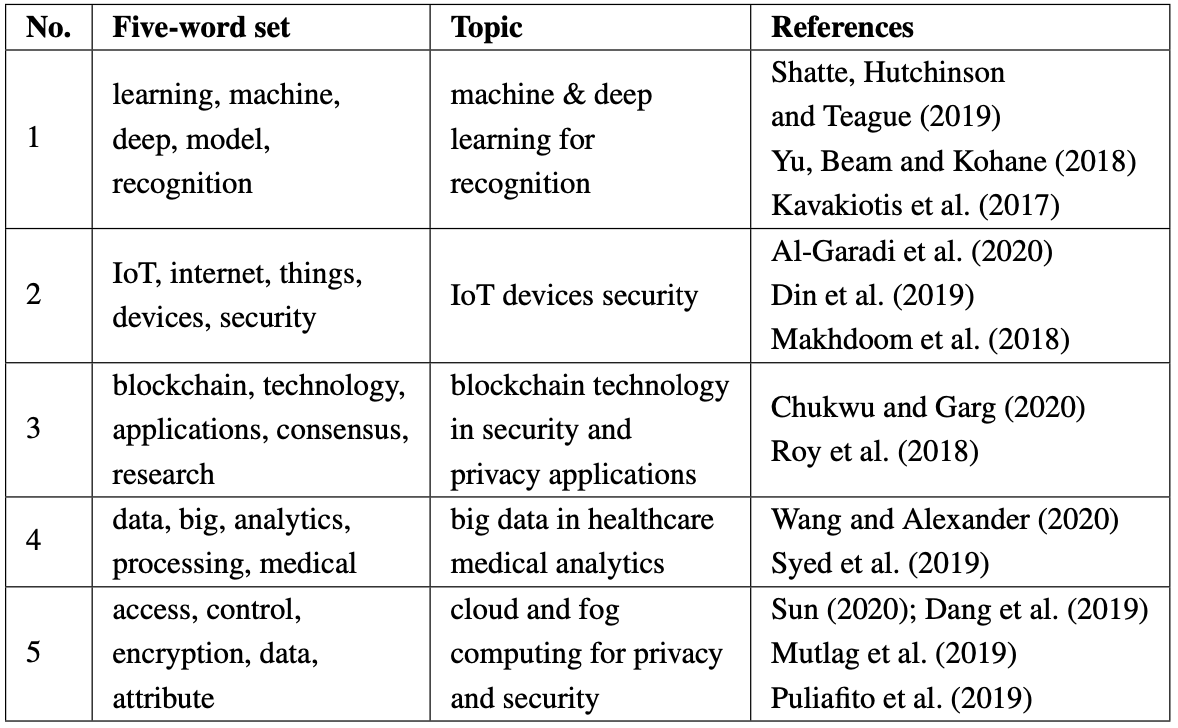
\includegraphics[width=1\textwidth]{figures/SR0008ES23/fig1.png}
        \caption{Topic modeling results obtained with the NMF algorithm in \cite{x249}.}
        \label{fig1:SR0008ES23}
    \end{figure}
    
    \textbf{Page 7:}
    Next is the total number of the papers reviewed (403) and the numbers of the papers in the searching groups.
    
    \textbf{Page 8:}
    Analisys of the e-health papers by the number of words.
    
    \textbf{Page 9:}
    The description of the prediction models in e-health was descriped in this page.
    
    \textbf{Page 10:}
    The studies with descriptive analysis was mentioned here.
    
    \textbf{Page 11:}
    Some management computational tools for unstructured data are show in this page.
    
    \textbf{Page 12:}
    Representing some data science arias such as data mining.
    
    \textbf{Page 13:}
    Mentioning the dufferent areas of the Artificial Intelligance.
    \begin{figure}[H]
        \centering
        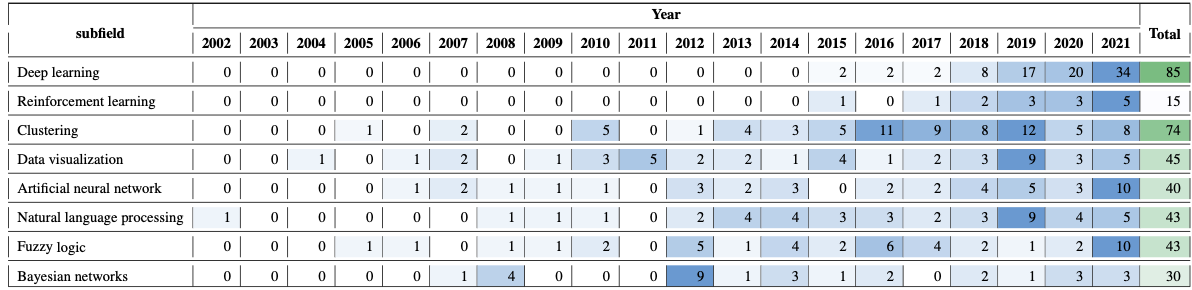
\includegraphics[width=1\textwidth]{figures/SR0008ES23/fig2.png}
        \caption{Number of e-health papers from \cite{x249}.}
        \label{fig2:SR0008ES23}
    \end{figure}

    \textbf{Page 14:}
    The authors intriduced a machine learning and the questions which arise when working with them.
    \begin{figure}[H]
        \centering
        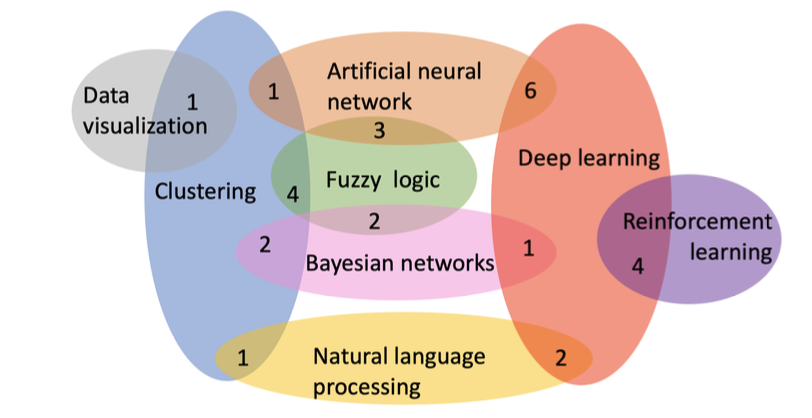
\includegraphics[width=.8\textwidth]{figures/SR0008ES23/fig3.png}
        \caption{Number of e-health papers from \cite{x249} venn diagram.}
        \label{fig3:SR0008ES23}
    \end{figure}
    
    \textbf{Page 15:}
    List of the papers which study or use machine learning techniques in e-health.
    
    \textbf{Page 16:}
    Introduction of data mining, NN, and natural language processing AI.
    
    \textbf{Page 17:}
    A particular applications of NLPs and best practisies in e-health for AI systems.
    
    \textbf{Page 18:}
    AI in: medical care, diagnostics, personalised medical care, ...
    
    \textbf{Page 19:}
    More AI applications in e-health: treatment optimisation, assistance or automated prescription, triage, surgery,pregnancy management.
    
    \textbf{Page 20:}
    AI in general hospital care: demant forcastig, screening, ...
    
    \textbf{Page 21:}
    ... epidemics prediction and flow analysis, fake news recognition.
    
    \textbf{Page 22:}
    AI for healthcare management: resource forcasting and managememt, grug chain supply, medical services scheduling, ...
    
    \textbf{Page 23:}
    ... facility allocation, preformance evaluation, brand management and marketing, finantial data, fraud detection, ...
    
    \textbf{Page 24:}
    ... patient satisfaction. AI work in lab dor COVID-19 vacseen development...
    
    \textbf{Page 25:}
    ... fluently transforms into AI tools to recognise fake news about COVID-19. Also the authors starts discuss other AI implementations...
    
    \textbf{Page 26:}
    On this page the insights and obsticles in the e-health with IA are outlined. The main diractions of AI implementation are cancer treatment, depression, Alzheimer disease, heart failure, and diabetes. To get full benefits from AI technology we need to overcome the defencivness and the learning curve for the profesionals in the healthcare industry and learn how to implement the AI systems flawlessly.

    \textbf{Page 27:}
    The Corona Virus crises gave a push for new data and analytical development.
    The deep learning models not just boost the performance of the healthcare services but also ensure the safety and integrity of the patient's data.
    
    \textbf{Page 28:}
    This page is all about legal regulations on the organisational and governance levels.

    \textbf{Page 29:}
    It is a need in setting people minds into all-sharing data to overcome the resistance barriar in sociaty. The next paragraph is about predicting and managing the future pandemics.
    
    \textbf{Conclusions:}
    The conclusion is played around the nessasity of beter data analysis and collection, since the machine learning models are already advanced in respect to the quality and quantity of the data resources.